\chapter{Theoretische Einführung}



\section{Grundlagen des 3D-Drucks mittels selektivem Laserschmelzen (SLM)}
	Die \emph{additive Fertigung} (AM) spielt in unserem Leben eine immer größere Rolle. Während
	sich bereits ein Hobbymarkt für preisgünstige 3D-Drucker im eigenen Haushalt etabliert hat,
	ist die industrielle Anwendung nicht zu vernachlässigen. Eine von Essentium, einem Hersteller
	von industriellen 3D-Druckern und Materialien, angefertigte Umfrage zeigte, dass sich die
	Anzahl der Firmen, die 3D-Druck zur industriellen Fertigung benutzen, von 2018 auf 2019 fast
	verdoppelte. Während der Anteil 2018 noch bei 21\% lag, änderte er sich innerhalb eines Jahres
	auf 40\% \cite{stevenson2019survey}.

	Obwohl es eine Vielzahl unterschiedlicher Methoden der additiven Fertigung gibt, funktionieren
	alle nach einem ähnlichen Grundprinzip: Das digitale 3-dimension\-ale Modell wird durch einen
	sogenannten \emph{Slicer} in Schnittebenen unterteilt, die vom 3D-Drucker nacheinander
	produziert und aufgeschichtet werden.

	%\subsection{Funktionsweise und Unterschiede zu anderen Methoden}
	\subsection{Funktionsweise und Unterschiede zum bekannteren FDM-Druck}
		Das vermutlich bekannteste Verfahren zur additiven Fertigung ist wahrscheinlich das
		\emph{Fused Depositing Modeling} (FDM), aus markenrechtsgründen auch bekannt als
		\emph{Fused Filament Fabrication} (FFF). Dabei wird ein Kunststofffilament aufgeschmolzen
		und durch eine Düse extrudiert. Die Düse (\emph{Hotend}) fährt hierbei während des
		extrudierens wie in Abbildung \ref{fig:fdm} dargestellt die Schnittebene ab, sodass
		Ebene für Ebene das gewünschte Objekt aufgeschichtet wird. Schichtdicken sind bei diesem
		Verfahren üblicherweise zwischen \SI{0,025}{\milli\meter} und \SI{1,25}{\milli\meter}
		\cite{wikipedia2021fused}.

		Obwohl dieses Verfahren relativ einfach umzusetzen ist wird es durch verschiedene Faktoren
		limitiert. So ist beispielsweise für die Qualität die Form des zu druckenden Objekts
		relevant. Außerdem ist dieses Verfahren auf bestimmte Materialien beschränkt, wie
		Thermoplaste und Formwachse. Die Druckbarkeit wird nicht zuletzt auch durch die
		Gravitation beschränkt, sodass je nach Form auch Stützstrukturen (\emph{support}, siehe
		Abbildung \ref{fig:fdm}) erforderlich sein können \cite{wikipedia2021fused}.

		\begin{figure}[ht]
			\centering
			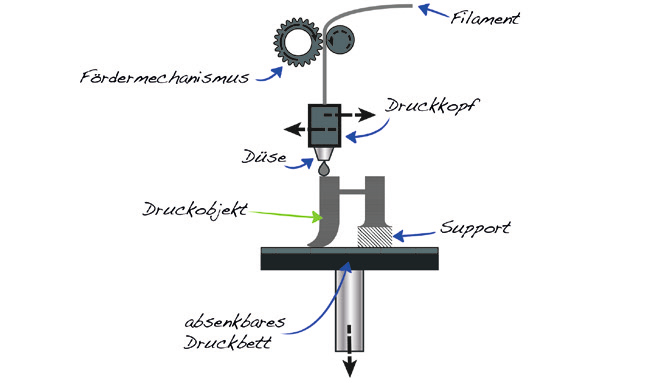
\includegraphics[width=0.9\textwidth]{chapter/main/img/fdm.png}
			\caption[Schematische Darstellung des FDM-/FFF-Verfahrens]{Schematische Darstellung
			einer möglichen Konfiguration des als FDM oder FFF bekannten 3D-Druck-Verfahrens. Ein
			Fördermechanismus schiebt das Filament durch eine aufgeheizte Düse. Durch eine
			Bewegung der Düse und/oder des Druckbetts in mindestens 3 Achsen erfolgt eine Formung
			des gewünschten Objektes Ebene für Ebene. \cite[S. 114]{horsch20143d}}
			\label{fig:fdm}
		\end{figure}

		Das in dieser Arbeit beobachtete Verfahren ist jedoch das \emph{selektive Laserschmelzen}
		(SLM). Der Drucker besteht hierbei aus zwei Gefäßen mit beweglichen Böden (Abbildung
		\ref{fig:slm_sls}). Das Gefäß für den Materialvorrat (\emph{feed container}) ist mit dem
		Material in Pulverform gefüllt, während das andere wenig bis gar nicht gefüllt ist. Beim
		Drucken einer neuen Ebene hebt sich der Boden des Materialvorrats und eine Walze
		(\emph{Beschichtungseinheit}) überträgt das dosierte Material in den Druckraum, dessen
		Druckbett abgesenkt wird. Ein beweglicher Laser fährt nun die gewünschte Schnittebene ab
		und verschmilzt das Pulver zu einer festen Form.
		\todo[color=red]{Quelle dazu finden bzw. nennen. Florian Horsch?}

		\begin{figure}[ht]
			\centering
			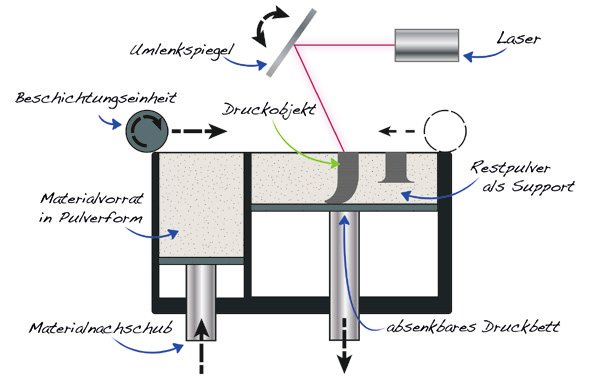
\includegraphics[width=0.9\textwidth]{chapter/main/img/sls_slm.png}
			\caption[Schematische Darstellung des SLM-Verfahrens]{Schematische Darstellung des
			SLM-Verfahrens. Der bewegliche Spiegel sorgt für eine präzise Positionierung des
			Laser-Punktes. Während sich der Boden des Vorrats\-gefäßes im Prozess anhebt, senkt
			sich der Boden des Druckraums ab. \cite[S. 119]{horsch20143d}}
			\label{fig:slm_sls}
		\end{figure}

		Das Druckbett wird üblicherweise um \SI{30}{\micro\meter} bis \SI{100}{\micro\meter}
		abgesenkt \cite{song2012effects}. Zu den am häufigsten verwendete Materialien, die beim
		SLM-Verfahren verwendet werden, zählen Titanlegierungen, insbesondere das in der Luft- und
		Raumfahrt populäre Ti6Al4V \cite{song2012effects,shi2016performance,brandl2012morphology}. % maybe sadali2020influence, too? but it refs brandl2012morphology
		Aluminiumlegierungen werden ebenfalls verwendet
		\cite[je Al-Si-10Mg]{yan2020comparative,zou2017study}.

	\subsection{Beobachtbare Defekte im fertigen Bauteil}
		\subsubsection{Porenbildung}
		Aufgrund verschiedener physikalischer Phänomene treten während des Verfahrens Vorgänge auf,
		die sich in Materialdefekten bemerkbar machen. Einer der bekannstesten Defekte ist die
		\emph{Porenbildung}. Mit einer Größe von weniger als \SI{100}{\micro\meter} zählen diese
		Gaseinschlüsse zu den kleinsten der hier aufgeführten Defekte \cite{zhang2017defect}. Es
		werden zwei verschiedene Gasquellen unterschieden. Während eine Quelle des dafür
		notwendigen Gases die Verdampfung mancher Legierungsbestandteile, wie beispielweise
		Magnesium, sein kann, kann ein Gaseinschluss nicht zuletzt auch durch Einschluss des beim
		Prozess verwendeten Umgebungsgases erfolgen \cite{galy2018main}. In letzterem Fall kann
		zum Beispiel eine zu geringe Packungsdichte des verwendeten Materialpulvers die Ursache
		sein. Das Gas dringt hierbei während des Schmelzprozesses in die Schmelze ein, erreicht
		aber aufgrund einer hohen Kühlrate die Oberfläche nicht vor dem Erstarren, sodass beim
		Erhärten des Materials ein Lufteinschluss die Folge ist. Aus diesem Grund haben Poren eine
		näherungsweise sphärische Form. Sie sind üblicherweise im im gefertigten Bauteil
		gleichverteilt aufzufinden. Das komplette Eliminieren aller Poren gilt als sehr schwer
		\cite{zhang2017defect}. Galy et al. zufolge hat die Porengröße und -form einen
		entscheidenden Einfluss auf die Qualität des Bauteils. Größere Makroporen verschlechtern
		die Qualität stärker als kleinere Mikroporen, wobei sich mehrere Mikroporen während einer
		Hitzebehandlung zu größeren Makroporen vereinigen können. Eine stärkere Entrundung der
		sphärischen Form der Poren kann eine Ursache von Rissen im Bauteil sein
		\cite{galy2018main}. Poren unterschiedlicher Größe sind in Abbildung
		\ref{fig:defects_porosities} zu sehen.

		\begin{figure}[ht]
			\centering
			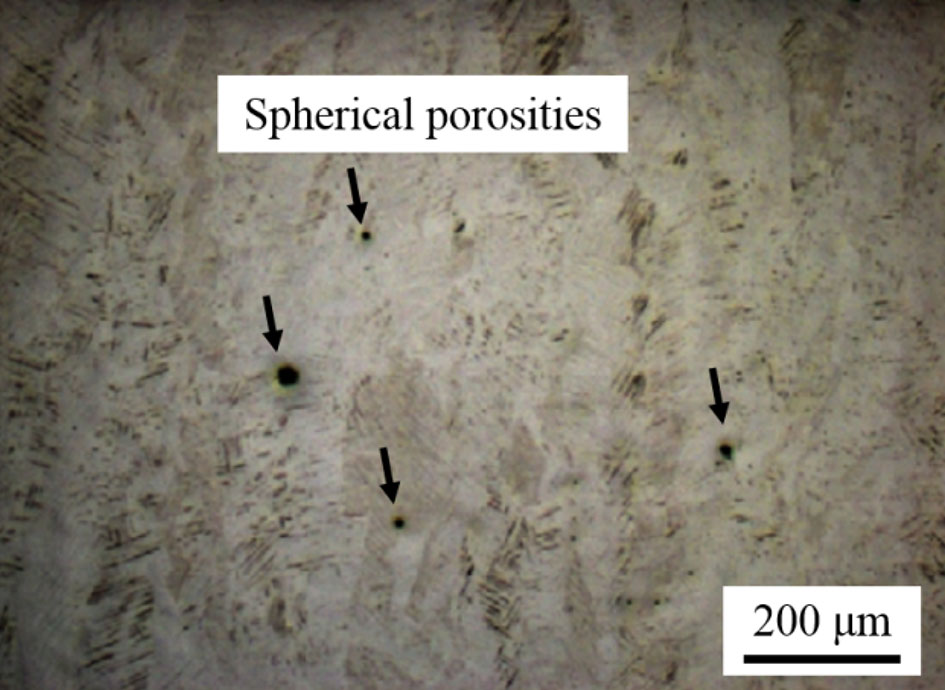
\includegraphics[width=0.7\textwidth]{chapter/main/img/defects/porosities.png}
			\caption{Poren sphärischer Form unterschiedlicher Größe entstehen durch Gaseinschlüsse
			\cite{zhang2017defect}}
			\label{fig:defects_porosities}
		\end{figure}

		\subsubsection{Mangelnde Verschmelzung}
		Eine mangelnde Verschmelzung (\emph{lack-of-fusion} oder kurz: \emph{LOF}) entsteht
		überwiegend durch unzureichende Energiezufuhr während des Schmelzprozesses. Durch die zu
		niedrige Energie vermindert sich die Breite des Schmelzbades. Bei unzureichender
		Überlappung der Bahnen kann dies zu fehlender Haftung zwischen diesen (sogenannten
		\emph{bonding defects} Abbildung \ref{fig:defects_lof} a)) führen. Außerdem resultiert
		die mangelnde Aufschmelzung in zahlreichen Pulvereinschlüssen (Abbildung
		\ref{fig:defects_lof} b)). Sollte die Energiezufuhr sogar unzureichend sein, um die
		gesamte Schichthöhe zu penetrieren, führt dies zu mangelhafter Bindung zwischen den
		Ebenen. Aus diesen Gründen sind Defekte die mangelnde Verschmelzung betreffend
		hauptsächlich zwischen den Bahnen einer Ebene und zwischen den Ebenen selbst zu finden. Da
		diese Defekte eine raue Oberfläche erzeugen, wird der Materialfluss der nächsten Ebene
		ebenfalls gestört, sodass Zwischenebenendefekte auftreten können, die graduell durch
		mehrere Ebenen propagieren und somit Defekte zur Folge haben, die sich über mehrere Ebenen
		erstrecken. Legierungen mit oxidierbaren Bestandteilen wie Al-Si-10Mg können durch einen
		entstehenden Oxidfilm und der damit verbundenen verminderten Benetzbarkeit ebenfalls
		Probleme mit der Aneinanderbindung von Bahnen haben \cite{zhang2017defect}.

		\begin{figure}[ht]
			\centering
			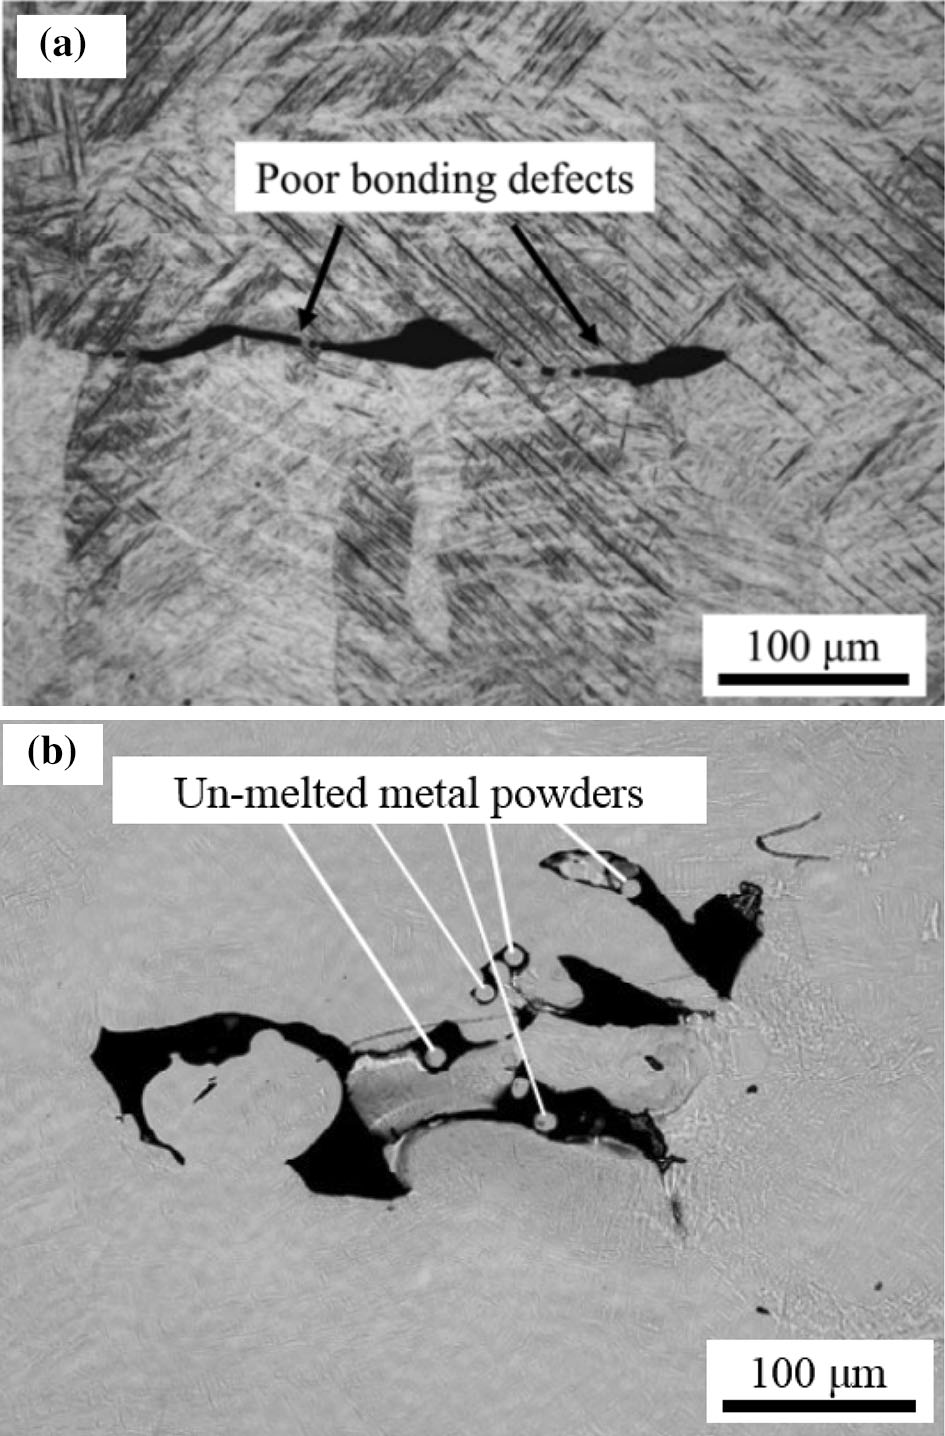
\includegraphics[width=0.7\textwidth]{chapter/main/img/defects/lack_of_fusion.png}
			\caption{a) Zwei Bahnen mit schlechter Verbindung durch mangelnde Überlappung
			b) Gut erkennbare Pulvereinschlüsse durch unzureichendes Aufschmelzen des Pulvers
			in Hohlräumen \cite{zhang2017defect}}
			\label{fig:defects_lof}
		\end{figure}

		\subsubsection{Risse}
		Während des Schmelzprozesses herschen nach dem Schmelzen Kühlraten von bis zu
		\SI{e8}{\kelvin\per\second}. Der dadruch entstehende Temperaturgradient und die damit
		verbundene unterschiedlich starke Kompression führt zu hohen Spannungen im Material.
		Diese Spannungen können nun dafür sorgen, dass Risse (\emph{cracks}) entstehen und dass
		diese weiter durch das Material propagieren. Abbildung \ref{fig:defects_cracks} zeigt gut
		verschiedene Stellen eines Risses, der sich an einer Oberfläche gebildet hat und weiter in
		das Bauteil hineinpropagiert ist \cite{zhang2017defect}. Wie bereits in Abschnitt
		\emph{Porenbildung} erwähnt können auch nicht-sphärische Poren besonders begünstigend auf
		die Rissbildung wirken \cite{galy2018main}.

		\begin{figure}[ht]
			\centering
			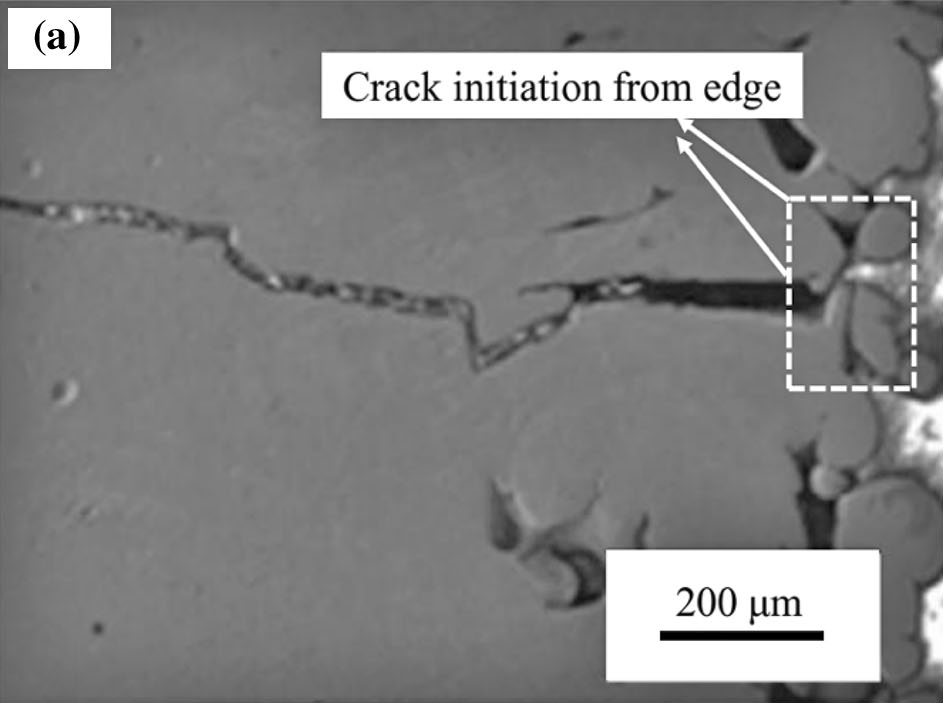
\includegraphics[width=0.7\textwidth]{chapter/main/img/defects/cracks_part.png}
			\caption{Aufnahme des Rands eines produziertes Objektes, von dem ein Riss ausgeht. Es
			ist gut erkennbar wie der Riss von Rand ausgehen in das Objekt hineinpropagiert ist.
			\cite{zhang2017defect}}
			\label{fig:defects_cracks}
		\end{figure}

	\subsection{Wichtige Parameter und Einfluss der Lasergeschwindigkeit}
		Beim SLM-Verfahren sind verschiedene Parameter einstellbar, die das Resultat in
		unterschiedlicher Weise und Stärke beeinflussen. Eine kategorische Übersicht über alle
		beim SLM-Prozess variierbaren Parameter ist in Abbildung \ref{fig:scheme_parameters} zu
		finden.

		\begin{figure}[ht]
			\centering
			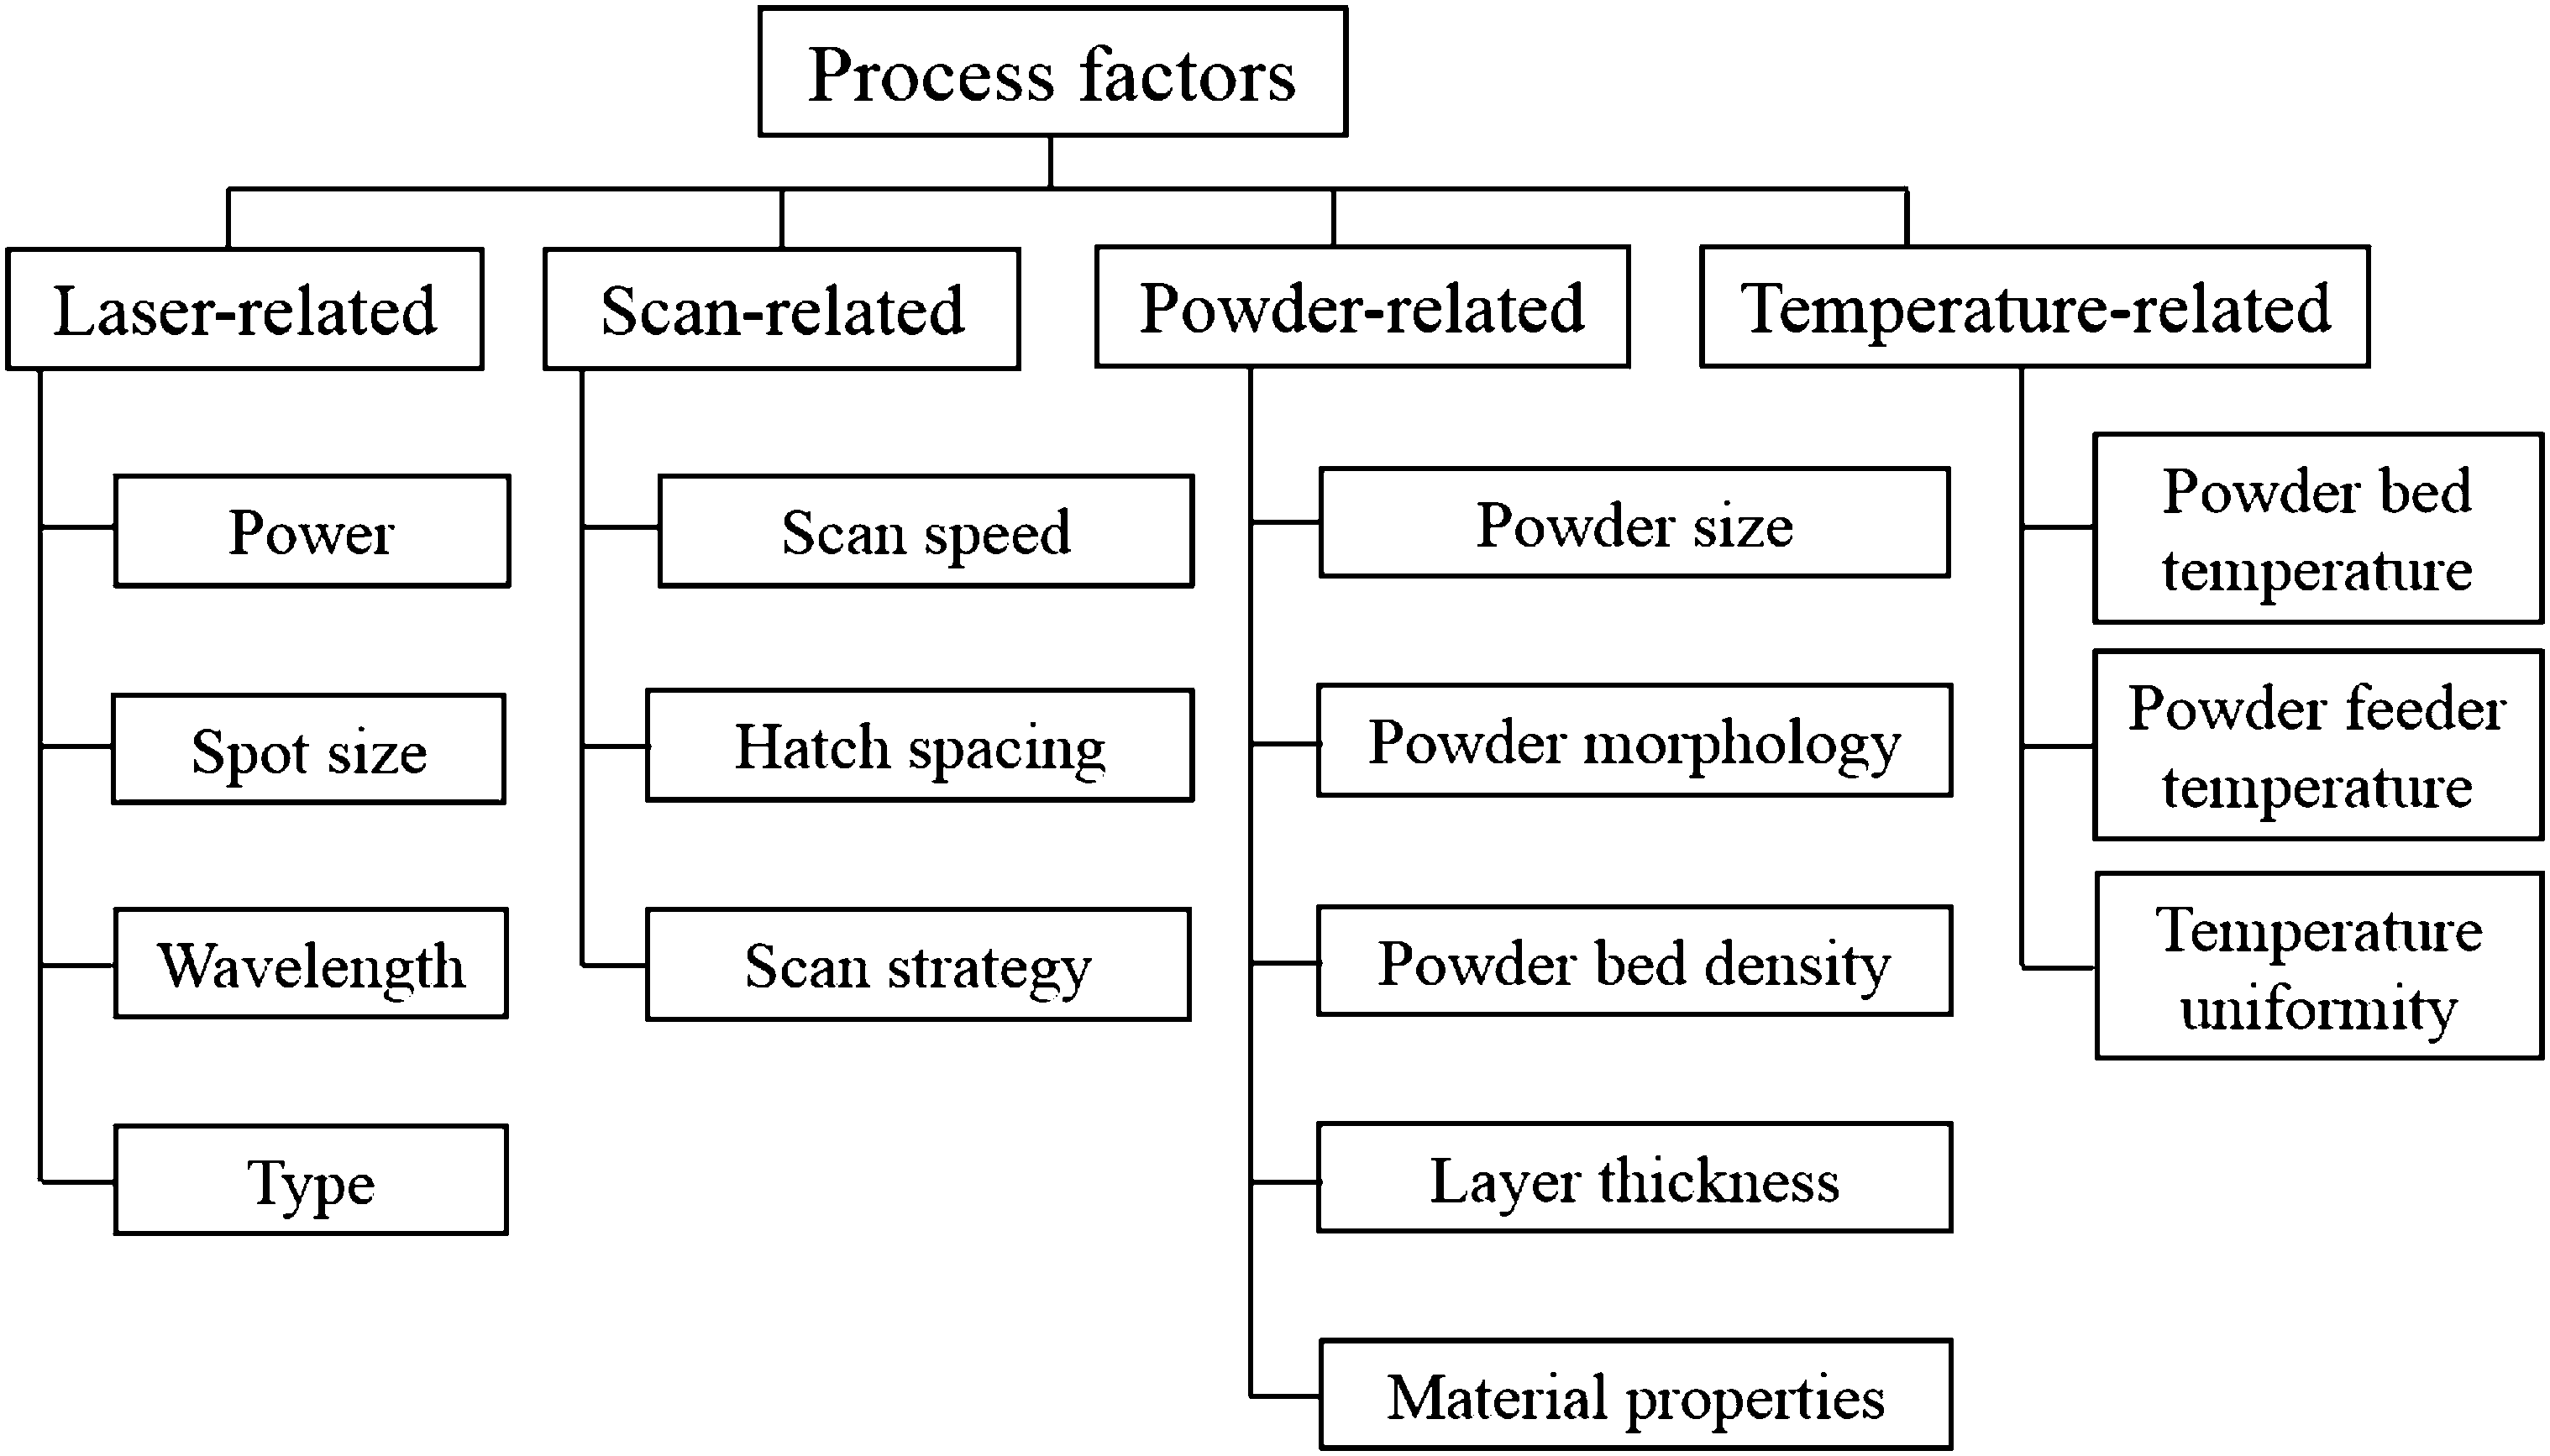
\includegraphics[width=\textwidth]{chapter/main/img/scheme_parameters_2.png}
			\caption{Eine Übersicht aller beim SLM-Verfahren einstellbaren Parameter nach
			Kategorie geordnet \cite{zhang2017defect,aboulkhair2014reducing}}
			\label{fig:scheme_parameters}
		\end{figure}

		Die wichtigsten Parameter sind, wie in Abbildung \ref{fig:slm_parameters} zu sehen, die
		Lasergeschwindigkeit (\emph{scanning speed}), die Laserleistung, der horizontale
		Bahnabstand (\emph{hatch distance} oder \emph{hatch spacing}), die Wellenlänge des Lasers,
		der Durchmesser des fokussierten Laserpunktes (\emph{spot size}) und die durch die Dicke
		der Pulverschicht bestimmte Ebenenhöhe (\emph{layer thickness})
		\cite{sadali2020influence}. Da für diese Arbeit die Größenordnung im Bereich der einzelnen
		Pulverpartikel von Interesse ist, werden im weiteren Verlauf der Bahnabstand und die
		Ebenenhöhe nicht weiter diskutiert.

		\todo[color=red]{Paper weiterlesen und verstehen, was zur Hölle da eigentlich abgeht?}

		\begin{figure}[ht]
			\centering
			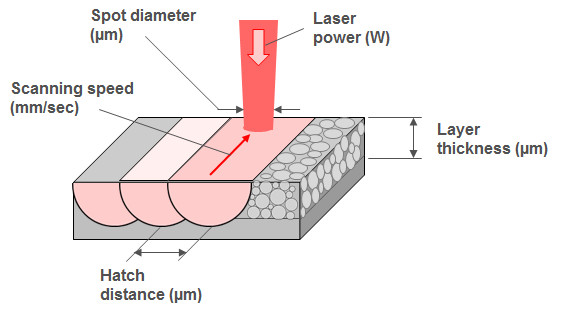
\includegraphics[width=0.8\textwidth]{chapter/main/img/slm_parameters.jpg}
			\caption{Darstellung und räumliche Einordnung der wichtigsten einstellbaren Parameter
			beim SLM-Druck und ihre üblichen Einheiten \cite{saunders2017x}}
			\label{fig:slm_parameters}
		\end{figure}


\section{Molekulardynamische Modellierung von SLM}
	\subsection{Numerische Integration von newtonschen Bewegungsgleichungen}
		Newtonsche Bewegungsgleichungen, die die Bewegungen für $N$ Teilchen wie in Gleichung
		\eqref{eq:newtone_dgl} beschreiben, können im Allgemeinen nicht immer analytisch gelöst
		werden.

		\begin{align}
			m_i \ddot{\uvec{x}}_i &= \sum_{\substack{j=0\\j \neq i}}^{N-1} \uvec{F}_{i,j}
			\label{eq:newtone_dgl}
		\end{align}

		Hierbei ist $m_i$ die Masse und $\uvec{x}_i$ der Ortsvektor des Teilchens $i$ und
		$\uvec{F}_{i,j}$ die vektorielle Kraft zwischen zwei Teilchen $i$ und $j$. Um dennoch eine
		Lösung der Bewegungsgleichungen zu erhalten bedarf es somit der numerischen Integration
		dieser.

		Die wohl simpelste Methode der numerische Integration ist das Euler-Verfahren. Hierbei
		wird das Taylorpolynom ersten Grades der Trajektorie verwendet und alle höheren Terme
		verworfen. Mithilfe der Diskretisierung des Zeitschritts \dt lässt sich von einem
		Integrationsschritt $n$ näherungsweise auf den nächsten $n+1$ schließen:

		\begin{align}
			\uvec{x}_{n+1} &= \uvec{x}_n + \dot{\uvec{x}}_n \dt + \BigO\left(\dt^2\right)
		\end{align}

		Das Problem, welches dem Euler-Verfahren innewohnt, ist trotz seiner einfachen
		Berechenbarkeit (oder gerade deswegen) die Tatsache, dass er nicht symplektisch ist und
		somit nicht die für ein solches System notwendige Forderung nach Energieerhaltung
		erfüllen kann \cite[S. 6f]{klein2013klassische}.


	\subsection{Grundlegende Funktionsweise der Molekulardynamik (MD)}

	\subsection{Notwendige Näherungen und Vereinfachungen}
		\todo[color=red]{Kleinere Skala und größere Gravitation mithilfe von \cite{glosli2007extending} motivieren.}
	\subsection{Implementierung des Laser}
	\subsection{Besonderheiten bei der Simulationssoftware IMD}
